\documentclass[DIN, pagenumber=false, fontsize=11pt, parskip=half]{scrartcl}

\usepackage{amsmath}
\usepackage{amsfonts}
\usepackage{amssymb}
\usepackage{enumitem}
\usepackage[utf8]{inputenc} 
\usepackage[ngerman]{babel} 
\usepackage[T1]{fontenc} 
\usepackage{pgfplots}
\usepackage{xcolor}
\usepackage{listings}
\usepackage{float}
\usepackage{graphicx}
\usepackage{svg}
\usepackage{booktabs}
\usepackage{gensymb}
\usepackage{dcolumn}


\definecolor{mygreen}{RGB}{28,172,0} % color values Red, Green, Blue
\definecolor{mylilas}{RGB}{170,55,241}

\newcommand{\norm}[1]{\left\lVert#1\right\rVert}

\lstset{language=Matlab,%
    %basicstyle=\color{red},
    breaklines=true,%
    morekeywords={matlab2tikz},
    keywordstyle=\color{blue},%
    morekeywords=[2]{1}, keywordstyle=[2]{\color{black}},
    identifierstyle=\color{black},%
    stringstyle=\color{mylilas},
    commentstyle=\color{mygreen},%
    showstringspaces=false,%without this there will be a symbol in the places where there is a space
    numbers=left,%
    numberstyle={\tiny \color{black}},% size of the numbers
    numbersep=9pt, % this defines how far the numbers are from the text
    emph=[1]{for,end,break},emphstyle=[1]\color{red}, %some words to emphasise
    %emph=[2]{word1,word2}, emphstyle=[2]{style},    
}

\title{Computer Vision I}
\author{Tim Luchterhand, Paul Nykiel (Group 17)}

\begin{document}
    \maketitle
    \section{Image Gradients}
    \subsection{}
    The sign of the sobel operator corresponds to the sign of the calculated gradient (linearity). By changing the sign the absolute value remains the same,
    the direction if the gradients gets rotated by $180 \degree$.
    \subsection{}
    \begin{table}[H]
        \centering
        \begin{tabular}{cccc}
            \toprule
            Position $v_i$ & $(I_x, I_y)$ & $\norm{\nabla I(v_i)}$ & $\sigma_i$ \\
            \midrule
            $v_1$ & $(255, -255)$ & $361$  & $-45\degree$ \\
            $v_2$ & $(765, -255)$ & $806$  & $-108\degree$ \\
            $v_3$ & $(255,  255)$ & $361$  & $45\degree$ \\
            $v_4$ & $(255,  765)$ & $806$  & $72\degree$ \\
            $v_5$ & $(1275,   0)$ & $1275$ & $0\degree$ \\
            $v_6$ & $(-765, 765)$ & $1082$ & $135\degree$\\
            \bottomrule
        \end{tabular}
    \end{table}
    \subsection{}
    \lstinputlisting{sh03ex01.m}
    \subsection{}
    \begin{figure}[H]
        \centering
        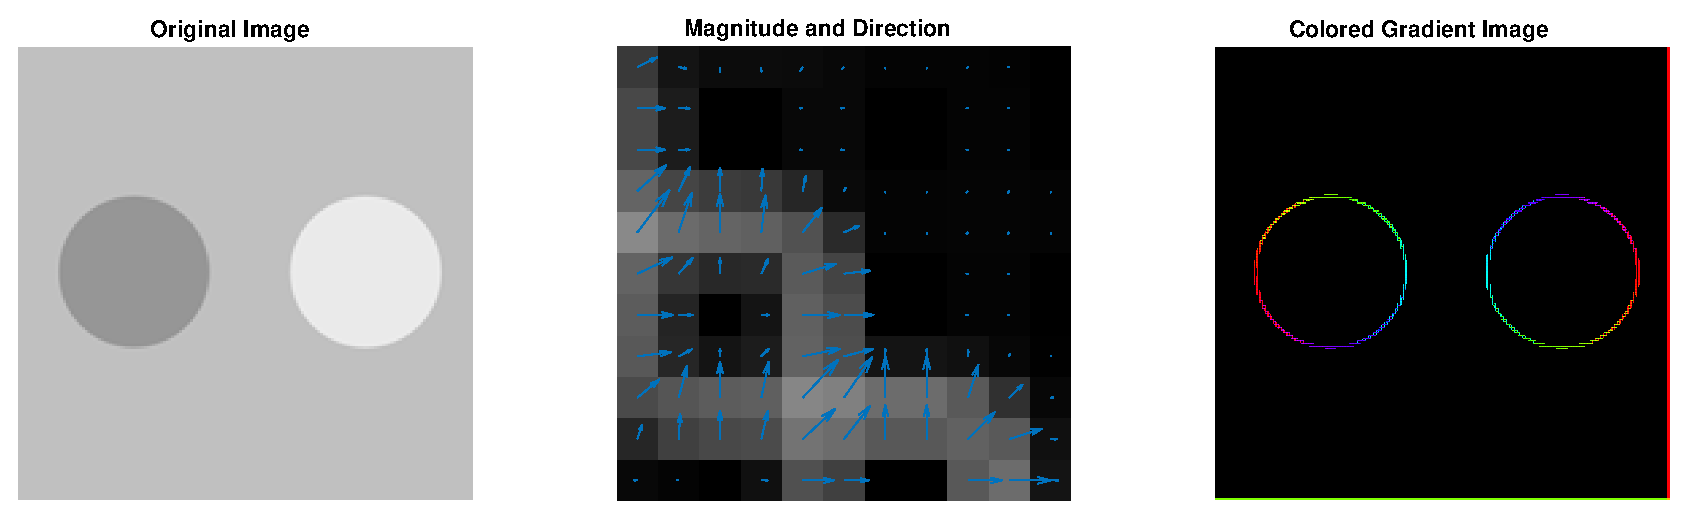
\includegraphics[width=\textwidth]{sh03ex01.eps}
        \caption{Output of the matlab script}
    \end{figure}

    \section{Deconvolution}
    \subsection{}
    \lstinputlisting{sh03ex02.m}
    \subsection{}
    \begin{figure}[H]
        \centering
        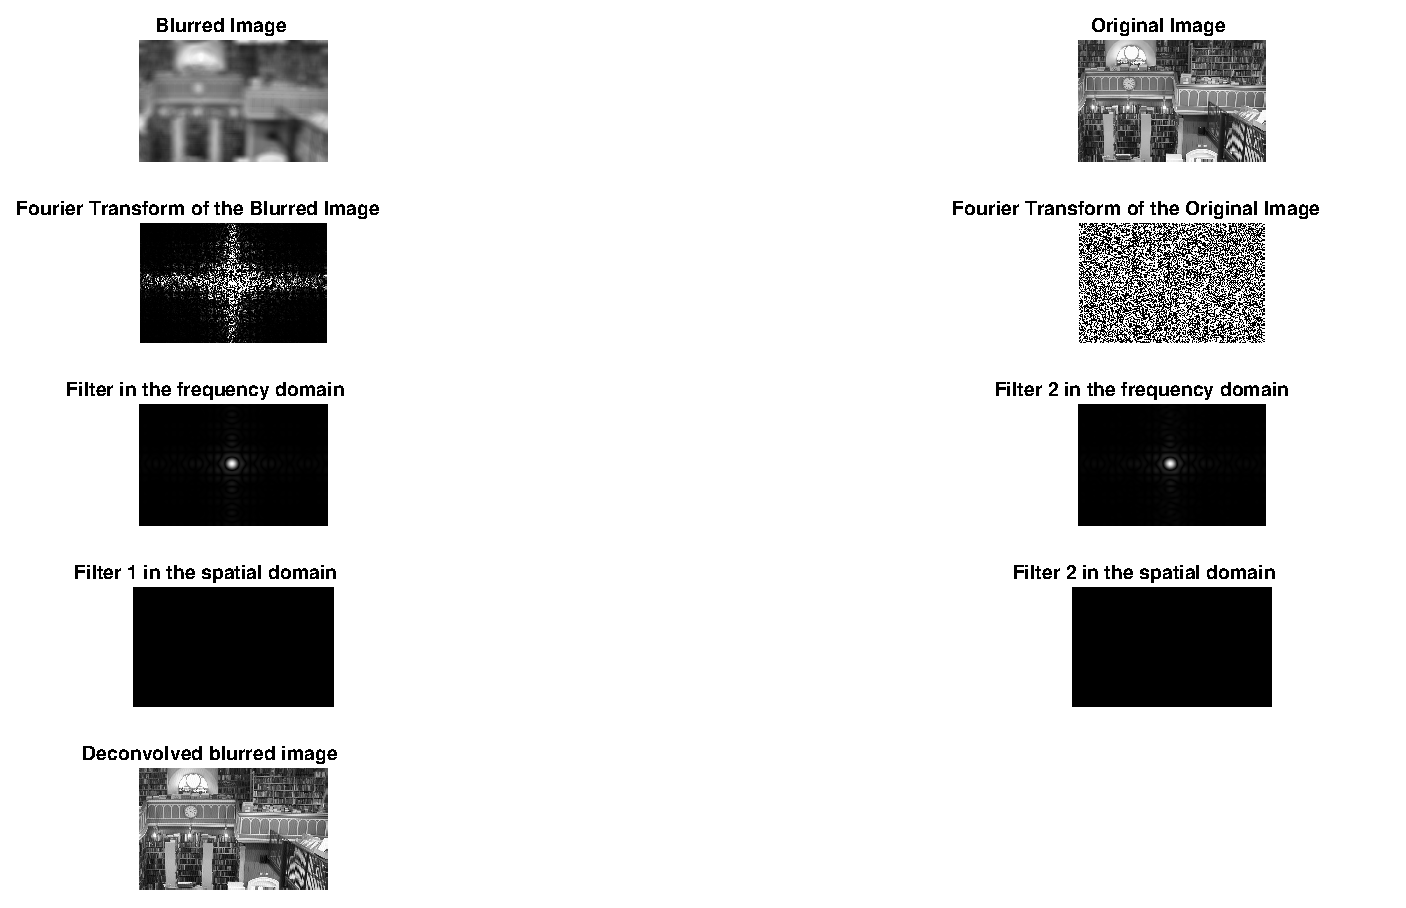
\includegraphics[width=\textwidth]{sh03ex02.eps}
        \caption{Output of the matlab script}
    \end{figure}
    \subsection{}
    If the original filter contains zeros in the frequency domain, the corresponding frequencies get surpressed and cannot be reconstructed.
\end{document}
